\documentclass[11pt]{article}
\usepackage[margin=1in, nohead]{geometry} 
\usepackage{amsmath}
\usepackage{amssymb}
\usepackage{accents}
\usepackage{graphicx} %package to manage images
\usepackage{wasysym}
\usepackage{wrapfig}
\usepackage{indentfirst} %Package to indent first paragraphs after new sections
\usepackage[compact]{titlesec} % Lots of Spacing Tools! If in doubt, default is good.
\usepackage[section]{placeins} % Prevents figures and other floats from drifting to a new section.
\usepackage[backend=biber, style=ieee]{biblatex}
    %\titlespacing{\section}{2pt}{0ex}{0ex}
    % \titlespacing{\subsection}{0pt}{0ex}{0ex}
    %\titlespacing{\subsubsection}{0pt}{0ex}{0ex}
    %\setlength{\parskip}{2pt}
    %\setlength{\parindent}{2em}
\linespread{1} % Sets Line Spacing
\setlength{\abovedisplayskip}{2pt} %Controls Above Equation Spacing
\setlength{\belowdisplayskip}{2pt} %Controls Below Equation Spacing
\usepackage{multicol}
 %Import the bibliography file

 %Prints bibliography

\pagenumbering{roman} % Hard shuts off page numbers if they are stuck on.
%% USEFUL PACKAGE SHORTLIST BELOW:
% \newenvironment{solution}
%  {\renewcommand\qedsymbol{$\blacksquare$}
%  \begin{proof}[Solution]}
%  {\end{proof}}
% \renewcommand\qedsymbol{$\blacksquare$}
% \usepackage{amsthm}
% \usepackage{lastpage}
% \usepackage{fancyhdr}
% \usepackage{tcolorbox}
% \usepackage{layout}
% \pagestyle{fancy}
% \setlength{\headheight}{40pt}
% \DeclareMathOperator\erf{erf}
% \graphicspath{ {./Images/} }
% \usepackage[rightcaption]{sidecap}
% \usepackage{braket}
% \usepackage{euscript} % add packages, settings, and declarations in settings.tex

\graphicspath{ {./images/}}

\addbibresource{references.bib}

\title{\textbf{\Huge{Remote Focusing}\\ \Large{An Exploration of Theory and Application to Microscopy}}}
\author{\Large{Alexander Marshall\thanks{The University Of North Carolina Department of Physics and Astronomy}}\\\Large{Optics 515}}
\date{\Large{May 1, 2024}}

\begin{document}
\maketitle
\tableofcontents
\newpage

%\begin{multicols}{2} %Sets up columns. Very helpful for documents with many equations.
\maketitle
\section{Theory of Remote Focusing}
\subsection{Introduction}
In microscopy, high-NA objectives are often associated with very narrow depth of focus, which in biological imaging is frequently much thinner than the region of interest in a given sample. One way to address this is to mechanically translate the objective (or sample) along the optical axis, thus moving the focal plane along with it. However, this process tends to be slow and difficult to integrate with other systems control, and in the case of fluorescence microscopy fails to decouple the excitation focal plane from the detection focal plane. Furthermore, the effective range of this adjustment is limited by the physical constraints of the stage and objective. If there were a way to adjust the focal plane without physically moving the objective or better yet without relying on mechanical translations at all, this would allow for far more rapid volumetric imaging.\par 
Remote focusing is a way to optically translate the focal plane of an objective without directly moving it. While there are other approaches to remote focusing \cite{Wilson}, in our lab we use tunable lenses conjugate to the back focal plane of the objective to achieve this without the physical translation of components. \cite{Hobson} This allows for rapidly adjusting the focal plane large distances within milliseconds, which has exciting applications in biological imaging. \cite{Annibale}  Introducing minimal aberration and magnification, it is an exciting tool which allows fast, automated three dimensional imaging. There are a diverse array of types of electronically tunable lenses, or ETLs. Our system uses Optotune electronically tunable lenses, which pass a user-specified current through a hydraulically-shaped meniscus, causing electromagnetic activation of the fluid. This causes a change in the fluid lens volume, altering the dioptric power of the lens. \cite{Chen} In our lab, we also use remote focusing in the excitation light-path to dynamically control the focal plane of our illumination beam, enabling advanced techniques such as total internal reflection or highly inclined swept tile fluorescence microscopy. To understand the theory behind this technique, I summarize the derivation of remote focusing via Fourier Optics, then analyze its behavior using geometric optics.

\subsection{Fourier Optics Approach}
This section closely follows the derivation performed by Zuo et al. \cite{Zuo} We start off with assuming our system is telemetric, which in this case means that refocusing avoids the introduction of additional phase-curvature across the field of view. This would result in the addition of variable magnification across the field of view. This is crucial, as otherwise data processing would be unduly arduous and under this assumption, we can model the propagation of the wavefunction $u_0$ modified by the free space transfer function $H$ as follows. 
\begin{equation}
	u_{\Delta z}(x,y) = \mathcal{F}^{-1}\left[ \mathcal{F}(u_0(x,y))H_{\Delta z}(u,v)\right]
\end{equation}
In brackets, we see that we have taken the Fourier transform of the wave to find its corresponding frequency-space function, and then modify that with the transfer function. In the paraxial approximation the free space transfer function is known to be
\begin{equation}
	H_{\Delta z}(u,\nu) = \exp\left[-i \pi \lambda \Delta z (u^2 + \nu^2)\right].
\end{equation}
\par Replicating the phase modification of free space via a spatial light modulator (SLM) represents the angular spectrum method and is widely used in holographic reconstruction due to its ability to produce an image field which does not vary in size along the optical axis. However, there are many practical difficulties of working with an SLM, so we instead utilize an electronically tunable lens (ETL). In Fourier optics, in the paraxial approximation a lens produces a transfer function of the form \cite{Goodman}
\begin{equation}
	t_l(x,y) =\exp \left[ - i \frac{k}{2f}\left(x^2 + y^2\right)\right].
\end{equation}
Since our ETL is in the spatial coordinates of the Fourier plane of the 4f system, it has a transfer function
\begin{equation}
	t_l(\xi, \eta) = \exp\left[ \frac{-i \pi}{\lambda f_c}\left(\xi^2 + \eta^2\right)\right].
\end{equation}
Notice that equation 4 is similar in form to the free space transfer function given in equation (2); by selecting a specific combined focal length $f_c$, we can do the equivalent of propagating the wave through free space some distance $\Delta z$. In our case, we use only a stand-alone ETL rather than a combined system, so $f_c = f_e.$ Converting from  spatial to frequency coordinates in the Fourier plane,  we can compare it to our known free space transfer function $H_{\Delta z}$ above and solve for axial translation as a function of the tunable focal length.
\begin{gather} 
		H_{\Delta z}(u,\nu)=t_l(\xi, \eta) \\
		\exp\left[-i \pi \lambda \Delta z (u^2 + \nu^2)\right]= \exp\left[ \frac{-i \pi}{\lambda f_e}\left((\lambda f u)^2 + (\lambda f \nu)^2\right)\right]\\
		%redundant! \lambda \Delta z (u^2 + \nu^2) = \frac{\lambda f^2}{f_e}(u^2+\nu^2)\\
		\Delta z = \frac{f^2}{f_e}
\end{gather}

\subsection{Ray Optics Approach}
In this section, we follow the derivation performed by Qu and Hu. \cite{Qu} When centered at the focal plane of two relay lenses rather than at the back focal plane, ETL3 also causes minor demagnification at high dioptric power. To see why this is, we turn to another paper which analyzes the impact of a remote focusing objective in the detection pathway in more detail. We begin with the thin lens equation
\begin{gather}
	\frac{1}{I} + \frac{1}{I'} = \frac 1 {f_O'}
\end{gather}
for $f_O'$ is the focal length of the objective, $I$ is the distance between the object and the objective and $I'$ is the distance between the objective and the image. Now let us assume that we have an ETL at the back focal plane of our objective. This ETL produces an axial translation of the focal plane $\Delta z$. This means we may now write a system of two thin lens equations to model the light going from the object plane, through the objective, to the BFP where the ETL is, and then to the imaging plane.
\begin{gather}
	\frac{1}{I-\Delta z} + \frac{1}{I_1'}  = \frac 1{f}\\
	\frac{1}{f -I_1'}+\frac{1}{I_2'} = \frac{1}{f_e'}
\end{gather}
The first thin lens equation models the system from the new object plane, which has been shifted by $\Delta z$ from the old object plane via remote focusing by the ETL, through the objective, and to the image after the objective at a distance of $I_1'$. The second thin lens equation models the system from the image after the objective through the ETL of variable focal length $f_e$ and to the second image after the ETL at a distance of $I_2'$. Due to the configuration of our system, the distance between the image after the objective and the objective is equal to the distance from the objective to the ETL at the back focal plane, which is the focal length, and the distance from ETL2 to the image after ETL2 where the camera is placed, so that
\begin{equation}
	I' = I_2' + f_O'.
\end{equation}
Now, we solve the system of equations given by 8-11 via MATLAB \footnote{Code available upon request} to find $\Delta z$.
\begin{equation}
	\Delta z = \frac{f^2}{f_e'}
\end{equation}
This result is similar to the result we got in equation 7, but here our objective is in the back focal plane of the system and $f$ is the objective's focal length, which is related to the magnification of our system. 
\par Let us pivot to considering a 4F system with two relay lenses and an ETL in the plane conjugate to the back focal plane. In our system, ETL2 and ETL3 are at the focal plane of two relay lenses conjugate to the back focal plane rather than in the back focal plane itself, so this will model a system analogous to ours. In this case, we get thin lens equations describing the transition from object through the objective to the image and from the intermediate image through the ETL to the detector
\begin{gather}
	\frac{1}{I-\Delta z}+\frac 1{I_1'} = \frac 1{f}\\
	\frac{1}{I' + f_r' - I_1'}+\frac1{I_2'} = \frac{1}{f_r'}
\end{gather}
where we maintain the same variable convention and introduce $I_2'$ is the distance between the image after the first relay lens and the relay lens and $f_r'$ is the focal length of the relay lenses. In this system, since the ETL is a distance $d_1$ from the relay lens, we get 
 \begin{equation}
	d_1 = I_2' + f_e'.
\end{equation}
The distance from the relay lens to the ETL is given by
\begin{equation}
	d_1 = f_r' + \frac{f_2'^2}{M_O' f}.
\end{equation}
Using MATLAB, we solve for $\Delta z$
\begin{equation}
	\Delta z = %\frac{(f_r' - I)^2}{f_e'^2 f^2}= 
	\frac{f_r'^2}{M_O'^2 f_e'}
\end{equation}
where $M_O' = (f_O'-I)/f_O'$ is the magnification of our system. We must also account for the fact that in our system, our ETLs are always in air so $n\approx 1$ while the objective is in an immersion media with some index $n$. Accommodating this \cite{Fahrbach} gives us our final expression for axial translation in an immersion media.
\begin{equation}
	\Delta z = \frac{nf_r'^2}{M_O'^2 f_e'}.
\end{equation}
While this configuration allows much less translation range than the back focal plane setup, it offers key advantages. Theoretically, the dioptric power of the ETL does not affect the magnification of the system in either the back focal plane or conjugate to the back focal plane. However, in practice it causes both demagnification and irregular spatial distortions in the image. While these issues are quite pronounced in the back focal plane setup, they are more limited in the relay lens setup and are negligible under low dioptric power. \cite{Qu}\cite{Fahrbach} Furthermore, the relay lens setup allows us to use two relay lenses in a fluorescent light microscopy setup, with one to translate the excitation pathway and the other to translate the emission pathway.

\section{Remote Focusing Example}
\subsection{Introduction to Optical System}
Our optical system \cite{Hobson}\cite{Liu} (see Figure 1) is designed for light sheet fluorescence microscopy, and has two paths which diverge at the dichroic mirror of a filter cube just after a shared objective. 
In our system, we have three identical electrically tunable lenses (Optotune, EL-10-40-TC-VIS-20D), two of which are used for remote focusing. \cite{Hobson} We control ETLs by passing a known current though each via a controller box (Optotune, ICC-4C) which is in turn controlled by custom LabVIEW software and Optotune Cockpit. The first, ETL 2, is responsible for remote focusing in the illumination light path, while the second, ETL3, is responsible for focusing in the detection light path. In our field of research, it is important to be able to translate the focal plane of the light sheet by a set amount using ETL2, while ETL3 must be able to move the imaging plane to the same location.  In order to use these devices as designed, we must therefore create a look up-table for each ETL, tying applied current to optical axis translation $\Delta z$. 
% NOT NEEDED: In the case of the illumination path, we will measure the beam waist of a light sheet in the focal plane, then define the Rayleigh length of the light sheet.
% OUT OF PLACE:
% Approximating the light-sheet as Gaussian in its thin direction, we will then use this information to translate the sample stage upwards in known increments, using the illumination ETL to keep it focused on the sample slide. I also wish to quantify the minimum beam waist of the light sheet at various optical displacements and compare it to the Abbe Diffraction limit and the Gaussian diffraction limits, as this is of interest to our experimental design for this system.\\

\subsection{Predictions}
In theory, the current $I \propto P_e$, where $P_e$ is the dioptric power of the lens $P_e = 1/f_{e}$. Defining $\Delta P_e \equiv P_{e-max}-P_{e-min}$, we can rewrite eq. 18 in terms of dioptric power for a more convenient form expressed as
\begin{equation}
	\Delta z = \frac{n \Delta P_e f_r'^2}{M_O'^2}.
\end{equation}
For our predictions, we assume each ETL has the manufacturer-guaranteed dioptric power range of $P \in [-10, 10] m^{-1}$ diopters, so $\Delta P_e = 20 m^{-1}.$ In practice, the dioptric powers of these lenses likely exceed these parameters, and the actual relationship between current and lens focal power is dependent on component temperature, but is highly replicable under relatively consistent lab conditions.

\par In theory, both the remote focusing ETLs follow equation 19. Since we have $f=125mm$ relay lenses \cite{Liu}, we get a predicted axial transfer range of $\Delta z={15625mm^2P_e}/{M_O'^2}$. This predicts a range of $\pm 591 \mu m$ for a 20X objective and $\pm 66 \mu m$ for a 60X objective. However, we may control only current applied to the ETL, which controls dioptric power. Dioptric power is dependent on both current and lens temperature. The non-ideal behavior of the ETL compounds with the non-ideal behavior of optics so that in practice, experimental behavior differs significantly from theoretical predictions. To ensure accurate axial control, we calibrate our ETLs under anticipated experimental conditions.

\par Going forward, it will be important to differentiate between the excitation focal plane, the sample plane, and the detection focal plane. The \textit{excitation} focal plane is the plane in which the beam waist lies, and is translated via altering the dioptric power of ETL2 or physically moving the objective. The sample plane is the physical location of the sample's surface, and is static for any given experiment. The \textit{detection} focal plane is the plane which is imaged on the CCD, and is translated via altering the dioptric power of ETL3 or physically moving the objective.

\subsection{ETL Calibration}
ETL2 is in the excitation pathway of our system. Using a light sheet, we will first focus the excitation beam into the sample plane via objective height adjustment and ETL2. We use a slide coated generously with fluorescent 200nm beads as our sample.
\par We use $\mu$Manager\cite{uManager} to move the microscope objective upwards in the Z direction in known discrete steps. We then bring this image into focus in the camera via ETL3 to adjust for the objective displacement and refocus the image. We then minimize the width of a Gaussian light-sheet by using ETL2 to translate the excitation focal plane back into the sample plane. Because we are compensating for a known displacement of the objective via ETL2, we can link the current value of ETL to focal-plane translation. Taking many of these steps allows us to map the relationship between ETL2 current and $\Delta z_{ex}$. So according to Equation 19, we predict maximum axial scanning range of $\Delta z = 1183nm$ over the full theoretical dioptric range. \par
ETL3 is in the detection plane of the microscope. To calibrate it, we follow much the same procedure we did for ETL2, but rather than involving the excitation pathway we simplify things using the built-in transmission illumination lamp and a calibration grid, allowing us to isolate the detection pathway. As before, we translate the objective by a known step, then compensating for the output with ETL3, moving the detection focal plane back into the sample plane and recording the current necessary to do so. In this way we can create a map of the relationship between ETL3 current and $\Delta z_{em}$.
% Below, paste the light sheet computations! But first, update them for the correct effective NA.
\subsection{Light-Sheet Characterization}
In this experiment, we use our ETLs to decouple the emission and excitation focal planes and use this image and characterize the profile of a light sheet. First, we use ETL2 to focus the light sheet in the sample plane, where we again use a slide with 200nm beads for our sample. Then we displace the objective by known increments, translating both the emission and excitation focal planes by $\Delta z$. Then we bring the beads back into focus using ETL3, moving the emission focal plane back into the sample plane. We then image the beam at some distance from its beam waist $\Delta Z.$ After doing this for a variety of objective displacements, we analyze the images to determine the beam waist as a function of axial displacement, $\omega(z)$. \par
We make several predictions about the light sheet. The beam waist in a LSFM system is given by \cite{Ernst}
\begin{equation}
    \omega_0 \approx \frac{0.85 \lambda}{2 NA}
\end{equation}
where NA is the numerical of the illumination objective and $\lambda$ is the excitation wavelength. Now, we must compute the ideal beam width and compare this with our own findings. For our 60X objective, which has an NA of $1.5$, and 561nm laser excitation light, we get $\omega_0 \approx 165nm.$ A beam simulator specifically designed for this purpose \cite{Remacha} verifies this result. This predicts a Full-Width at Half Max of 193$\mu m$. For an approximately Gaussian light sheet, the Rayleigh length is
\begin{equation}
	Z_R = \frac{\pi \omega_0^2}{\lambda}
\end{equation}
so we should expect a Rayleigh length of around 152nm. To process my data, I used FIJI \cite{Fiji} to rotate my image until the light sheets were vertical in the image and created a histogram of intensities by column. Then I added offset Gaussian fits to each plot and exported the data.
\section{Results and Discussion}
\subsection{ETL Calibration Results}
\par To analyze the results, we put the focal plane position to ETL current pairings into Excel and graphed them. We then created a linear best fit function for each, then extrapolated the maximum value for -10 to 10 diopters, then computed the difference between these two values to find the maximum $\Delta Z$. For a 60X objective ETL2, we got $108\mu m$ $\Delta Z$ range. For ETL3, we get $166.6 \mu m$, which is somewhat larger than anticipated. This is not really surprising; Optotune lenses are designed to exceed their rated dioptric power by some margin under most conditions.
\par Using the 20X objective, %honesty hour--I'm not sure if it was ETL2 or ETL3!
 we obtained a scanning range of $1065\mu m$ for ETL3. This is again somewhat less than the predicted axial range, but is approximately 9 times the 60X scanning range, as predicted by equation 19.
\subsection{Light Sheet Characterization} %duplicated from longer write up
Our beam waist minimized at $0.5 \mu m$ according to raw data and at $0.7\mu m$ for the Gaussian best fit curve. I found the Rayleigh length $Z_R\approx 2 \mu m$. Note that this value has a lot of error in it, as our stage is able to move in only $1\mu m$ increments, so our resolution is quite limited here. Our light sheet width is a factor of around three (raw intensity profile) to five (gaussian fit) times thicker at the beam waist than anticipated. The Rayleigh length for a beam of this width is predicted to be $1.4 \mu m$ and $2.74 \mu m$ for $\omega_0 \approx 0.5 \mu m$ and $0.7 \mu m$ respectively. Thus, while our beam waist was significantly larger than predicted for our theoretical beam, our Rayleigh length was close to the predicted value for a sheet of the observed width.
\subsection{Discussion}
The entire Hestia system remains under active development, as is known to currently have alignment imperfections. This may be causing some of the irregularities in ETL performance. Currently, there is no implementation of an algorithmic autofocus function implemented for either ETL, so each of these calibrations was performed using a protocol utilizing human judgement, and there was some variability in the assignment of ideal current levels, even for identical objective positions. This manual process was time consuming, limiting the amount of data acquired. At some point, we hope to develop a more standardized method for this which leads to more replicable data and less noise. \par
Additionally, the light sheet characterization was not conducted using advanced image deconvolution or analysis. The beads used for this sample were 200nm in diameter, which is large compared to the theoretical beam waist as well as potentially causing scattering. All of these factors probably contributed to a larger-than-predicted beam waist measurement and in the future, more advanced data analysis techniques using MATLAB, image deconvolution using point spread functions, and 40nm beads will be implemented to improve precision.
\par Overall, the remote focusing system performed quite close to expectations, and appeared highly linear and predictable proximal to 0mA. Since we plan to use this system to image macrophages, a depth of $10 \mu m$ of axial scanning range is sufficient for our application. The calibration curves are very linear near equilibrium, and so this will likely perform well for our application.\par
It should also be noted that the beam shifts a lot as ETL2 is adjusted. This indicates that there is a lot of tilt in the light sheet, i.e. the excitation beam is not parallel with the primary optical axis, and is therefore not perpendicular to the imaging plane. This is surely increasing the apparent width of the beam and likely changes the behavior of the remote focusing as well. The emission pathway is likely not tilted in the same way, so this may be one reason for the difference in ETL2 and ETL3 performance.

%\section{Junk!}
%In our 4F setup, we use optical lenses are the relay lenses of our 4F system, which have $f = 125mm$. Plugging this into equation 8 and 10, in a system without magnification we get $\Delta z = \frac{15625 mm^2}{f_{ETL}}.$ Our ETL (Optotune 10-40) has an effective focal power range of -10 to 10 diopters. Dioptric power is given by $f_{ETL} = \frac{1m}{D}$ and therefore for us ranges from $f_{ETL} = (-\infty, -10]\cup [100, \infty)$ millimeters. This gives us a z-translation range of
% \begin{gather}
%	\Delta z = [-156.25, 156.25]mm.
% \end{gather}
% REMOVE ME
% Note that this change in our focal plane $\Delta z$ is defined in the magnified object field, which means that this is only valid for a non-zero magnification objective. The axial focal shift in the object-plane is given by
%\begin{gather}
%	\frac{\Delta z}{M^2},
%\end{gather} 
%so for a 60X objective we get $\Delta f = [-43.4, 43.4] \mu m$. Likewise, for a 40X objective, we get $[-97.7, 97.7] \mu m$, and for a 20X objective, we get $[-391, 391 \mu m]$. Whg % Note that we also have a 125mm lens going into a 200mm tube lens, which gives an effective magnification of 8/5. I'm not quite sure what to do with this.\\
%But we have yet to account for the magnification of our system, which we do below.
%In practice, however, I predict that the ETLs will have slightly different properties, since ETL2 occurs \textit{before} the objective in the illumination light path, while ETL3 occurs \textit{after} the objective in the detection light path. Theoretically, this shouldn't matter much, but with imperfect alignment and non-ideal optics, I predict there will be small differences in their behavior. Furthermore, based on the literature, I predict that the lenses will behave worse at high dioptric power, and that high ETL3 dioptric power will cause minor image demagnification.
% CITE Grewe, B.F., et al., Fast two-layer two-photon imaging of neuronal cell populations using an electrically tunable lens. Biomed Opt Express, 2011. 2(7): p. 2035-46.
\newpage
\newpage
\section{Gaussian Beam Power Transmission Through an Aperture}
\fbox{\begin{minipage}{\textwidth}
\textbf{Summary\\ For a Gaussian Laser beam, the power of a beam transmitted through an aperture $P_R$ is dependent on beam waist $w(z)$, the radius of the aperture $R$, and the total power of the beam $P_0$ as follows:}
\setcounter{equation}{0}
\begin{equation}
    P_R = P_0 \left[1-\exp{\left(\frac{-2R^2}{w(z)^2}\right)}\right]
\end{equation}
\end{minipage}}
The function given above may be derived from a Gaussian function as follows. (It may also be verified by digging through the Wikipedia page on Gaussian beams. See https://en.wikipedia.org/wiki/Gaussian\_beam\\\#Power\_and\_intensity.) A generic 2D Gaussian, such as a Gaussian laser's intensity distribution, is given by 
\begin{gather}
    f(x,y) = e^{-x^2 - y^2}.
\end{gather}
More generally, it may be written as 
\begin{equation}
    f(x,y) = A \exp \left[-\left(\frac{(x-x_0)^2}{2\sigma_x^2} + \frac{(y-y_0)^2}{2\sigma^2_y} \right)\right]
\end{equation}
In the case of a laser, let us a assume that the beam is radially symmetric and centered about the origin. Then we may write:
\begin{gather}
    f(x,y) = A \exp \left[-\left(\frac{x^2+y^2}{2\sigma^2}\right)\right]
\end{gather}
Lets integrate this from negative infinity to infinity to find the total power of the laser.
\begin{gather}
    P= A \int^\infty_{-\infty} \int^\infty_{-\infty} A \exp \left[-\left(\frac{x^2+y^2}{2\sigma^2}\right)\right] dx dy\\
    P = A \int^{2\pi}_{0} \int^{\infty}_{0} \exp \left[-\left(\frac{r^2}{2\sigma^2}\right)\right] d\theta \, r dr\\
    P = 2\pi A \int^{\infty}_{0} \exp \left[-\left(\frac{r^2}{2\sigma^2}\right)\right] \, r dr
\end{gather}
More generally, we can find the power of the laser passing through an aperture of radius $R$ by integrating from 0 to $R$.
\begin{gather}
       P = 2\pi A \int^{R}_{0} \exp \left[-\left(\frac{r^2}{2\sigma^2}\right)\right] \, r dr
\end{gather}
This integral may be solved without too much fuss via complex analysis, but for the sake of convenience I use the identity given by equation 3.321.4 in \textit{A Table of Integrals, Series, and Products, 8th Edition} by Daniel Zwilliger:
\begin{gather}
    \int^b_0 r e^{-ar^2} dr = \frac{1-\exp\left(-a^2b^2\right)}{2a}.
\end{gather}
Using this identity, we see that
\begin{gather}
    P_R = 2\pi A \sigma^2 \left[ 1-\exp(-\frac{R^2}{2\sigma^2})\right]\\
    P_{full} = \lim_{x\to\infty} P_R  = 2\pi A \sigma^2 [1]
\end{gather}
In defining this, we have assumed that the intensity profile, rather than the full power, is fixed. This isn't really useful to a fixed-power laser application: we want to find percentage of set power which passes through a certain radius. We therefore substitute the expression for full power into the expression for relative power.
\begin{gather}
     P_R = P_{full} \left[ 1-\exp\left(-\frac{R^2}{2\sigma^2}\right)\right]
\end{gather}
By convention, it is useful to talk about beam waist $w$, which is a diameter rather than the standard deviation we used, which is a radial measurement. Using $w=2\sigma$, we see that
\begin{gather}
    P_R = P_{full} \left[ 1-\exp\left(-\frac{2R^2}{w^2(z)}\right)\right].
\end{gather}
$\mathcal{Q}.\mathcal{E}.\mathcal{D}.$\\
Let us assume our infinity-focused Gaussian laser beam has a Rayleigh length much longer than the optical path of our system, so that $w(z)\approx W_0$. Then we can find the beam waist of our laser to be
\begin{gather}
    1-\frac{P_R}{P_0} = \exp{\frac{-2R^2}{W_0^2}}\\
    \ln{\left( 1-\frac{P_R}{P_0}\right)}=\frac{-2R^2}{W_0^2}\\
    W_0 = \sqrt{\frac{-2R^2}{\ln{\left( 1-\frac{P_R}{P_0}\right)}}}
\end{gather}
Then we may plug our measured values for Hestia in. For apetures along the light path of $\diameter = 0.9mm, 3.6mm$, we obtain power outputs $P_R/P_0 =  .24mW/2.5mW$ and $2.0mW/2.5mW$ respectively. Both these values predict $w_0=4.01mm$.\\
Also, the maximum intensity of a beam as a function of $z$ is given by \\
\subsection{CORRECTED BEAM WAIST}
    At current settings, the beam diameter is 1.536mm. Computations are as follows for an unrestricted beam of 0.761mW and a beam restricted through an aperture with diameter of 1.0mm with a power of 0.435mW. This results in 
    \begin{equation}
        W_0 = \sqrt{\left( \frac{-2*0.5^2}{ln\left[1-(.435/.761)\right]}\right)}
    \end{equation}
    So that $ 2W_0 = 1.536mm$. This time, I was very cautious to optomize the transmission of my beam through the aperture.
\begin{gather}
    I(0,z)= \frac{2P_0}{\pi \left(\omega(z)\right)^2}
\end{gather}
while the beam waist as a function of z is given by
\begin{gather}
    \omega_0 = \sqrt{1+\left(z/z_R \right)^2}
\end{gather}
where the Rayleigh length is
\begin{gather}
    z_R = \frac{\pi \omega_0^2 n}{\lambda}
\end{gather}
\newpage
\section{Gaussian Approximation of the Beam Waist}
Recall that previously, we used two diameters and the Gaussian power transmission through an aperture to find (in both cases) what our predicted beam width is $W_0=4.00mm$. Now, given an infinity-focused beam (i.e. Rayleigh length $>>1$) of a given width, we should be able to compute the new beam waist at the focal plane after it has passed through a lens using the following equation (Fundamentals of Photonics, 2nd ed., 3.2-13)
\begin{gather}
    W_0'= \frac{W_0}{\sqrt{1+(z_0/f)^2}}\\
    z' = \frac{f}{1+(f/z_0)^2}
\end{gather}
Note in our case, the Rayleigh length of the Gaussian laser beam $z_0>>1$, so we can instead use 3.2-17 to see
\begin{gather}
    2W_0' \approx \frac 4 \pi \lambda F_\#\\
    2W_0' \approx \frac 4 \pi \lambda \frac f D\\
    2W_0' \approx \frac 4 \pi \lambda \frac f {\diameter_{BFP}}
\end{gather}
I'm not certain what to implement for the excitation beam waist at the BFP. Our beam waist throughout the optical system is 
At the focal plane of the 125mm lenses, we have
\begin{gather}
    2W_0' \approx \frac 4 \pi \lambda \frac{125mm}{2(4mm)}\\
    2W_0' \approx 20 \lambda\\
    2W_0' = 22.3 \mu m
\end{gather}
for 561nm light. This would be easy to test via implementing a pinhole and checking to see if the power percentage transferred through the aperture is consistent with anticipated power transmission through a pinhole.\\
For for a 60X TIRF objective with a 200mm tube lens, we can do the Focal Length by doing $F_{TL}/M = 200mm/60 = 3.33mm$ so lets just go with 3.3mm. So we have something like this:
\begin{gather}
    2W_0' \approx \frac 4 \pi \lambda \frac{3.33mm}{2(4mm)}\\
    2W_0' \approx .297 \mu m
\end{gather}
Note that with a different formulation
\begin{gather}
    W_0' = \frac{f \lambda }{\pi W_0} 
    W_0' = \frac{3.33mm*561nm}{\pi 4mm}
    W_0' = 148.7 nm
\end{gather}
so we are being consistent at least. This seems unreasonably small, so that either our effective beam waist is far too large or something else odd is going on. \\

Note we have another possibility: using the Abbe diffraction limit as done above.
\begin{gather}
    \omega_0 \approx \frac{0.85 \lambda}{2 NA_{eff}}
    \omega_0 \approx 165nm
\end{gather}
This is a bit wider than we anticipated, but not as wide as we may have hoped. But here we have assumed that $NA_{eff} \approx NA_{theoretical}$ which may not be true. We need to find a more reasonable NA value. But how may we do this? I think one way is to shine a point in the BFP and see what comes out (angle wise). I think another is to assume that the LS is as wide as the effective NA allows it to be and see how that turns out. (Although this assumes a lot about the light sheet being effectively 1 point thick at the BFP.)
$NA = n\sin(\theta)$ so if we find the length of the LS we can figure out the effective NA. A quick gut check shows that we go between 10-105um for the LS height, so around 95 microns across. This gives an effective angle (arctan(a) = 47.5um/3.33mm)



Note, however, that this is the $W_0$ which is defined as the point where the intensity of the beam has fallen to $1/e^2$ of its maximum. Lets convert to $W_{FWHM}$ to make things simpler. We know that for Gaussian Beams, $W_0=0.843218*FWHM$, so $FWHM = .176\mu m$.
Its necessary to point out that Chad claims (and I'm sure he is correct) that \textbf{Gaussian Optics does not hold for objectives}. He does some rather complicated math to attain:
\begin{gather}
    FWHM_A=4.81 \mu m\\
    FWHM_L = 771nm
\end{gather}
for a Gaussian lightsheet in the axial and lateral directions respectively.
Chad sites the following in his computations (see p41 of his thesis).
    Wolf, E., Electromagnetic Diffraction in Optical Systems .1. An Integral Representation of the Image Field. Proceedings of the Royal Society of London Series a-Mathematical and Physical Sciences, 1959. 253(1274): p. 349-357.
203. Richards, B. and E. Wolf, Electromagnetic Diffraction in Optical Systems .2. Structure of the Image Field in an Aplanatic System. Proceedings of the Royal Society of London Series a-Mathematical and Physical Sciences, 1959. 253(1274): p. 358-379.
204. Chon, H.S., et al., Dependence of transverse and longitudinal resolutions on incident Gaussian beam widths in the illumination part of optical scanning microscopy. J Opt Soc Am A Opt Image Sci Vis, 2007. 24(1): p. 60-7.

 \newpage
\section[]{Fiolka Light Sheet Beam Waist Method}
subsection{FIOLKA Lightsheet Computations}\\
Note the primary source for this work is Fiolka's Lightsheet literature review. The beam waist in a LSFM system is given by 
\begin{gather}
    \omega_0 \approx \frac{0.85 \lambda}{2 NA}
\end{gather}
    Where NA is the NA of the illumination objective and $\lambda$ is the excitation wavelength. The lateral beam radius is given by 
    \begin{gather}
        \omega(x) = \omega_0 \sqrt{1 + \left(\frac{x}{x_R}\right)^2}\\
        x_R = \frac{n \pi \omega_0^2}{\lambda}
    \end{gather}
    where $x_R$ is the Rayleigh length in the lateral direction.
    In the y-direction, the beam is essentially of infinite width and thus limitless depth of focus, as this is the broad side of the sheet. The only limitation here is the optical train componenets.\\
    The lateral resolution of LSFM (i.e. in the x-y plane) is defined by 
    \begin{gather}
        \Delta r = \frac{\lambda_{em}}{2 NA_{det}}
    \end{gather}
    for the emission and detection wavelengths. This is because this is the FWHM radius of the beam, which is the point at which two airy disks would reach their first trough and be distinguishable.\\
    The axial resolution is given by the product of the illumination and detection point spread function, which in turn depend on the excitation and emission wavelengths adn the NA of the objective (which in our case is combined). In general, thinner light-sheets are generated by higher NA objectives with higher axial resolution but also have narrower Rayleigh lengths and thus worse field of view. In other words, it is messy, but can be approximated (assuming $NA_{exc}=NA_{ill}$) by
    \begin{gather}
        \Delta z \approx \left( \frac{2 NA_{ill}}{\lambda_exc} + \frac{n (1-\cos \theta)}{\lambda_em}\right)^{-1}
    \end{gather}
    where $\theta$ is the half-angle of the detection objective
    \begin{gather}
        \theta = \arcsin\left(\frac{NA}{n}\right)
    \end{gather}
    Now, we must compute the ideal beam width and compare this with our own findings. For our TIRF objective, which has an NA of and 561nm laser light,
    \begin{gather}
        \omega_0 \approx \frac{0.85\cdot561nm}{2*(1.5)}\\
        \omega_0 \approx 158.95nm
    \end{gather}
We can also use a beam simulator to verify our result--see https://github.com/remachae/beamsimulator. We end up with a main lobe width of .32$\mu m$, which is equivalent to $\omega_0=160nm$; our answer checks out.\par
Notice we also have a lateral \cite{Ernst} resolution limit of 
\begin{gather}
    \Delta r = \frac{\lambda_{em}}{2 NA_{det}}
    \Delta r = .187 \mu m
\end{gather}
\subsection{Considering a Tilted Light-Sheet}
We have to keep in mind that our light sheet is actually at some non-trivial angle. Considering the beam at an angle $\theta$, we consider the measured beam waist $W_0'$ to be the hypotenuse, the actual beam waist $W_0$ (i.e. what we would see if the beam were aligned vertically) is offset by some angle $\theta$, and the transverse distance traversed over the beam's angled path is orthogonal to the actual beam waist. We then have 
\begin{align}
    \cos \theta = \frac{W_{0}}{W_0'}\\
    W_0 = W_0' \cos \theta 
\end{align}
Note that the entire beam is being shifted upwards by translating the objective, so that as long as the angle of the beam approaching the objective is very small (and it certainly ought to be) there is not any sort of trigonometric consideration regarding the pre-objective beam angle. Now, we can correct for the beam waist.
\subsection{Examining a tilted light-sheet in the back focal plane}
Consider a beam entering the back focal plane. In order to make a light sheet, the beam must form a band following a narrow linear path across the BFP of the objective. In order to avoid lateral tilt, it must be centered in its narrow axis. If such a beam fully fills the back focal plane of the objective, it will create what is essentially an X, with all of the rays converging to the focal plane. Such a light-sheet cannot, however have any angle orthogonal to its length, because such a tilt is caused by being offset in one direction or another. Instead, it merely fills the entire possible azimuthal angle domain $\theta \in [-\theta_{max},\theta_{max}]$, where $\theta_{max}$ is the maximum possible angle allowed by $NA=\eta \sin \theta$. In other words, our light sheet is maximally angled, but is in the form of an upright hourglass rather than a tapering ramp. This is useless for reducing background, as we always will have a lot of background below the beam waist-focal plane intersection. In order to have a shape of the form $/|$ or something similar, the beam must be trimmed in the back focal plane so that we can angle both the bottom line and the top line, such that 

$\theta \in [\theta_1, \theta_2]$ for $0<\theta_1<\theta_2$ to form a tapering inclined ramp style light-sheet. In this case, we have an effective NA given by
\begin{equation}
    NA_{eff}=1.51 \sin (\theta_1-\theta_2).
\end{equation}
so that 
\begin{equation}
    w_0 = \frac{.85 \lambda}{2NA_{eff}}.
\end{equation}
From this, we can compute a new Rayleigh length
\begin{gather}
    Z_R = \frac{\pi w_0^2}{\lambda}\\
    Z_R = \frac{\pi (0.85)^2 \lambda}{4 (NA_{eff})^2}\\
    Z_R = \frac{\pi (0.85)^2 \lambda}{4 \left(1.51 \sin (\theta_1-\theta_2)\right)^2}\\
\end{gather}
So if we need the light sheet to be about $10 \mu m$, we can findings
\begin{gather}
    10\mu m = \frac{\pi (0.85)^2 \lambda}{4 (1.51 \sin (\theta_1-\theta_2))^2}
\end{gather}
\subsection[]{Tokunaga}
From Tokunaga, we see that
\begin{gather}
    R = dz \tan \theta
\end{gather}
for $R$ is the thickness of the light sheet's cross section with the coverslip.
To acquire a beam waist of the desired size at $\theta \approx 70^\circ$, which gives us $dz \approx 3.64 \mu m$.  Tokunaga gives 
\begin{gather}
    x=n  \times f_{obj} \times \sin \theta
\end{gather}
as his way of obtaining the angle $\theta$.
When $R / \tan \theta $ is small, Tokunaga notes $dz$ inflates more than predicted due to divergence of the illumination at the specimen, so to reduce this Tokunaga implements a field stop conjugate to the specimen plane. In order to minimize divergence at the edges of the field stop, it is conjugate to the specimen plane instead.
We can use simple gaussian beam propogations to determine the beam waist at a given location in the optical system. See my excel sheet for more information.\newpage
\section{Fluorescence Math}
Let $I(\lambda)$ be equivalent to the cuumulative intensity of the image at the CCD while $Q(\lambda)$ is the quantum efficiency of the CCD. Then by integrating the efficiency times the intensity of the image over some timescale and the spectrum detectable by the sensor, we get:
\begin{gather}
    I(\lambda) = \Delta T [P(\lambda) Ex(\lambda) A D Fl(\lambda) Em(\lambda) I(\lambda) + N_{Optical}(\lambda)]\\
    C = \int_0^t \int_{\lambda} Q(\lambda) I(\lambda) d\lambda dt + N_{Readout}
\end{gather}
We now must define some sort of reasonable estimate for $I(\lambda)$. We start out with the power emission spectra of the fluorescence LED as a function of wavelength, $P(\lambda)$. We then multiply this by the fraction of light transmitted by the excitation optical train, including all mirrors, filtersets, and objectives, $T_{ex}(\lambda)$. The product of $F_{ex}(\lambda)$ and $P(\lambda)$ gives the true excitation spectrum $X(\lambda)$ at the fluorophore. We then muliply this by single fluorophore cross sectional factor $A$ and concentration factor $D$, finding the excitation's effective effect modifier on the specimen. In other words, the excitation power is given by 
\begin{equation}
	X(\lambda) = P(\lambda) T_{ex}(\lambda)
\end{equation}
Now, we know that the emission of the fluorophore $M$ is a function of both wavelength and the excitation spectrum, which in turn is a function of wavelength. Let $M_{eff}(\lambda)$ be the fluorescence efficiency factor as a function of excitation wavelength. So we have 
\begin{equation}
	M(\lambda, X(\lambda))  = X(\lambda) M_{eff}(\lambda) 
\end{equation}
Technically speaking this is all a function of wavelength; every function so far is a simple pairing of power (or factor giving the percentage of power transmitted) to wavelength. However, it is confusing to incorporate all of the excitation function into the emission function implicitly. It is better represented by examining the efficiency of the fluorophore and the excitation spectrum separately. Basically, all of this is just to say that $X(\lambda)$ determines the excitation at the specimen and $M_{eff}(\lambda)$ represents the fluorophore. We therefore have that the light emitted is
\begin{equation}
	M(\lambda)  =P(\lambda) T_{ex}(\lambda) M_{eff}(\lambda).
\end{equation}
Now, for the emitted light to get to the camera detector, we need to pass through the detection path. Let's represent the transmission of the detection pathway as $T_{em}(\lambda)$. Then the amount of emission power reaching the camera $I$ is given by the product of the emission transmission and the light emitted.
\begin{gather}
	I(\lambda) = T_{ex}(\lambda) M((\lambda)\\
	I(\lambda)= P(\lambda) T_{ex}(\lambda) M_{eff}(\lambda) T_{em}(\lambda)+N_{Optical}
\end{gather}
Where $N_{Optical}$ represents the optical noise present in experimental setups. \\

We now have to convert from the image at the CCD to the digital signal we actually capture for data analysis. Firstly, the camera has several effects. A monocolor sCMOS effectively integrates the signal over the detectable wavelength spectrum and has a quantum efficiency, $Q(\lambda)$, which varies across it's operating range. sCMOS cameras also have some amount of eletronic background noise (also called readout noise) $N_{Readout}$. To convert to a digital signal $C$, we integrate over the emission light times the camera's efficiency with respect to wavelength and time to get an expression for our digital signal as
\begin{gather}
	C = \int Q(\lambda)I(\lambda) d\lambda dt + N_{Readout}.
\end{gather}
So our entire expression may be written as 
\begin{gather}
   C = \iint Q(\lambda) \left(P(\lambda) T_{ex}(\lambda) M_{eff}(\lambda) T_{em}(\lambda)+N_{Optical}\right) d\lambda dt + N_{Readout}
\end{gather}
This is a bit nasty. However, if we use a laser to excite the fluorophores, things simiplify greatly. Assuming a known amount of laser power at $\lambda = \Lambda$, we see
\begin{gather}
            C=  \iint Q(\lambda) \left( T_{ex}(\Lambda) M_{eff}(\Lambda) T_{em}(\lambda)+N_{Optical}\right) d\lambda dt + N_{Readout}.
\end{gather}
This saves us from having to figure out the spectrum of excitation light at the specimen. In theory, this would be a simple measure of plugging a known excitation source into FPbase with the excitation filters and seeing the output, but in practice this could be quite hard since I can't find the Prismatix data. It also heads off any wavelength-dependent stokes shift phenomena and reduces our excitation mess to a simple measurement of the laser in the BFP of the objective followed by multiplying by an efficiency factor for the emission efficiency rather than integrating over some sort of list of values. So effecitvely,we can boil all of those excitation terms into some constant $K$.
\begin{gather}
            C=  \iint Q(\lambda) \left(K * T_{em}(\lambda)+N_{Optical}\right) d\lambda dt + N_{Readout}.
\end{gather}


\section{Figures}
\begin{figure}
    \centering
    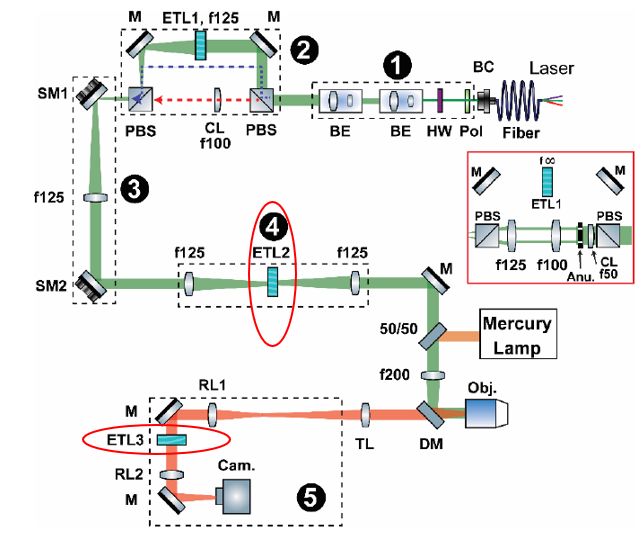
\includegraphics[scale=.50]{system.png}
    \caption[]{This figure, adapted from Liu et al \cite{Liu} with the permission of the corresponding author, depicts the optical design of our system. The ETLs used for remote focusing (circled in red) are at the focal planes of the 4F system, which are conjugate to the back focal plane of the objective.}
\end{figure}
\begin{figure}
    \centering
    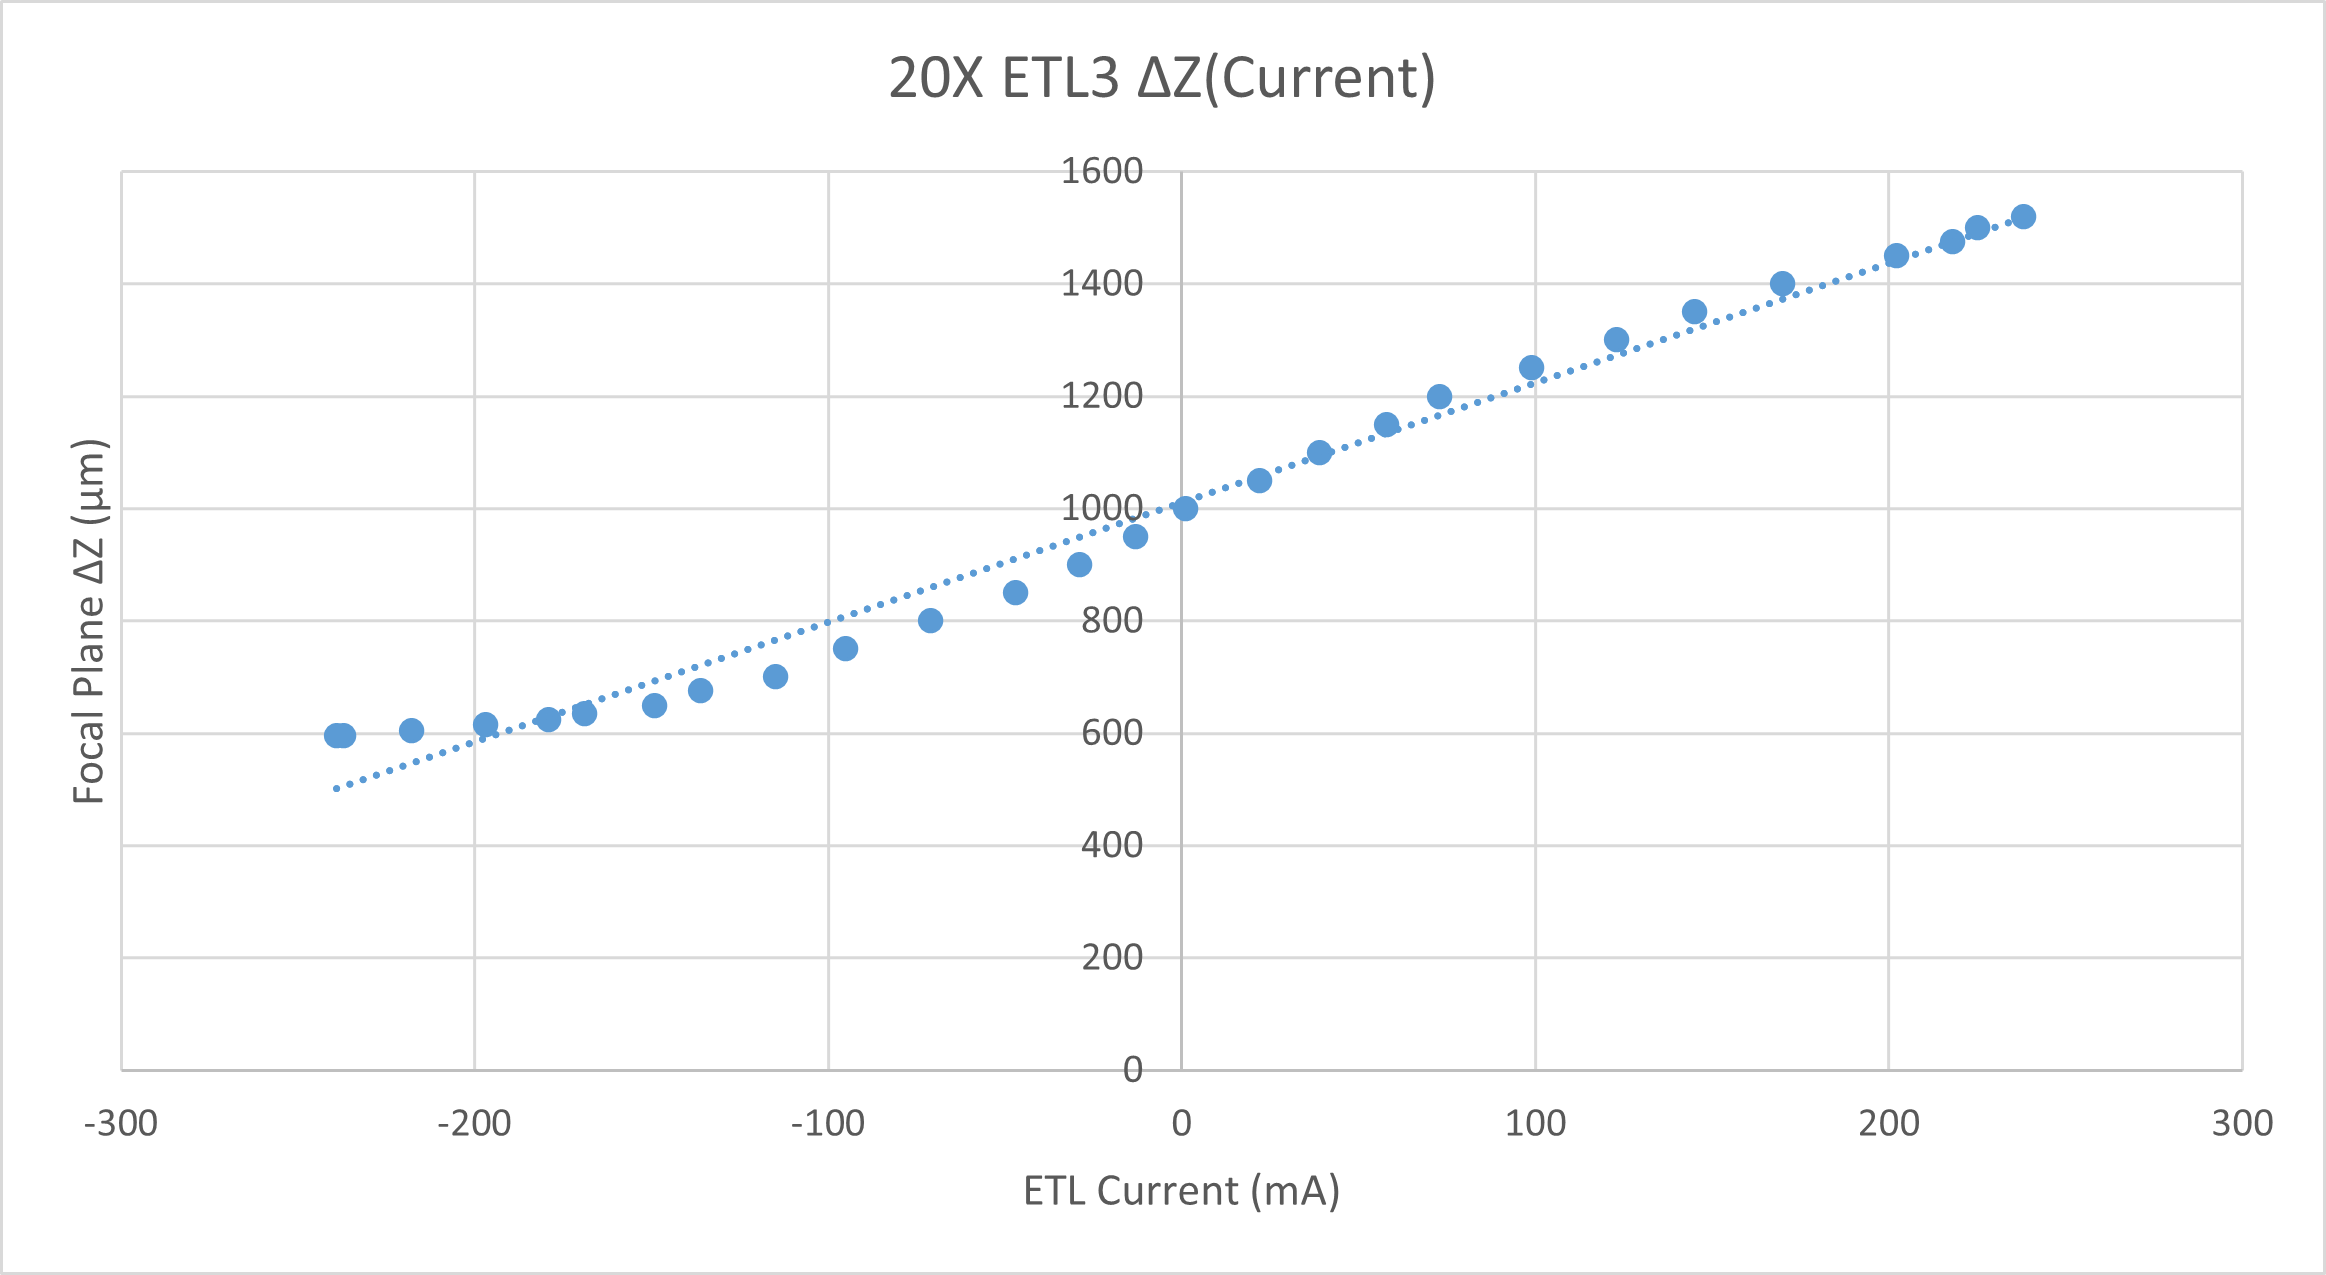
\includegraphics[scale=.75]{20XGraph.png}
    \caption[]{This graph depicts the relationship between ETL3 current and absolute focal plane position. Note the significant breakdown of linearity at large negative currents corresponds to major demagnification and spatial distortion of the image.}
\end{figure}
\begin{figure}
    \centering
    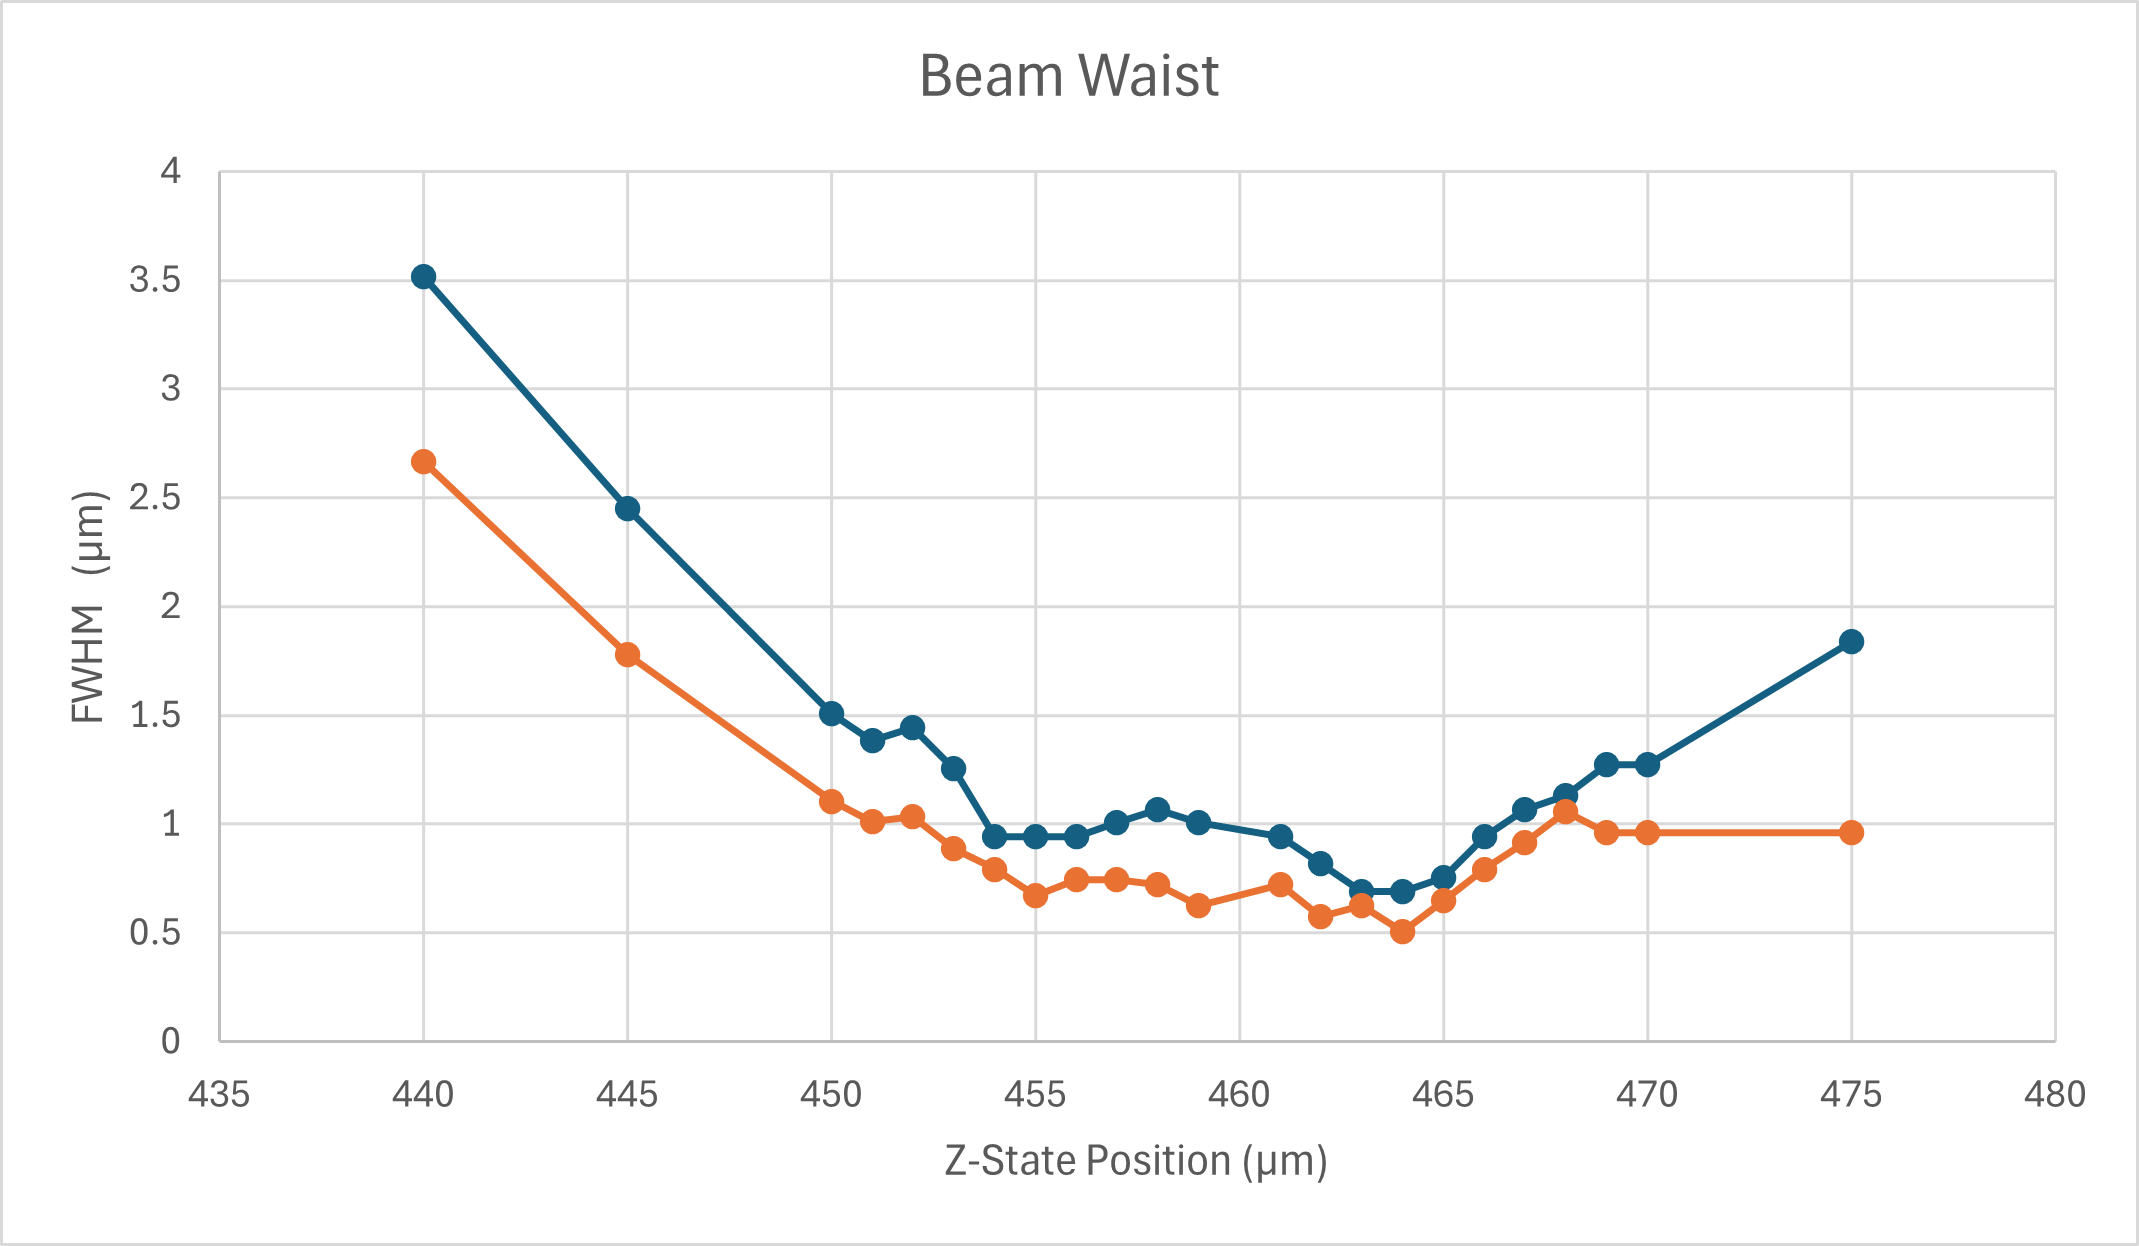
\includegraphics[scale=.75]{BeamWaist.png}
    \caption{This graph depicts the beam waist at a given objective position. The objective used is a 60X Olympus objective. ETL3 was used to keep the beads in focus via remote focusing, allowing us to profile the beam. The red line is the FWHM according to the raw data, while the blue line shows the FWHM of a Gaussian best fit of the data.}
\end{figure}
\begin{figure}
    \centering
    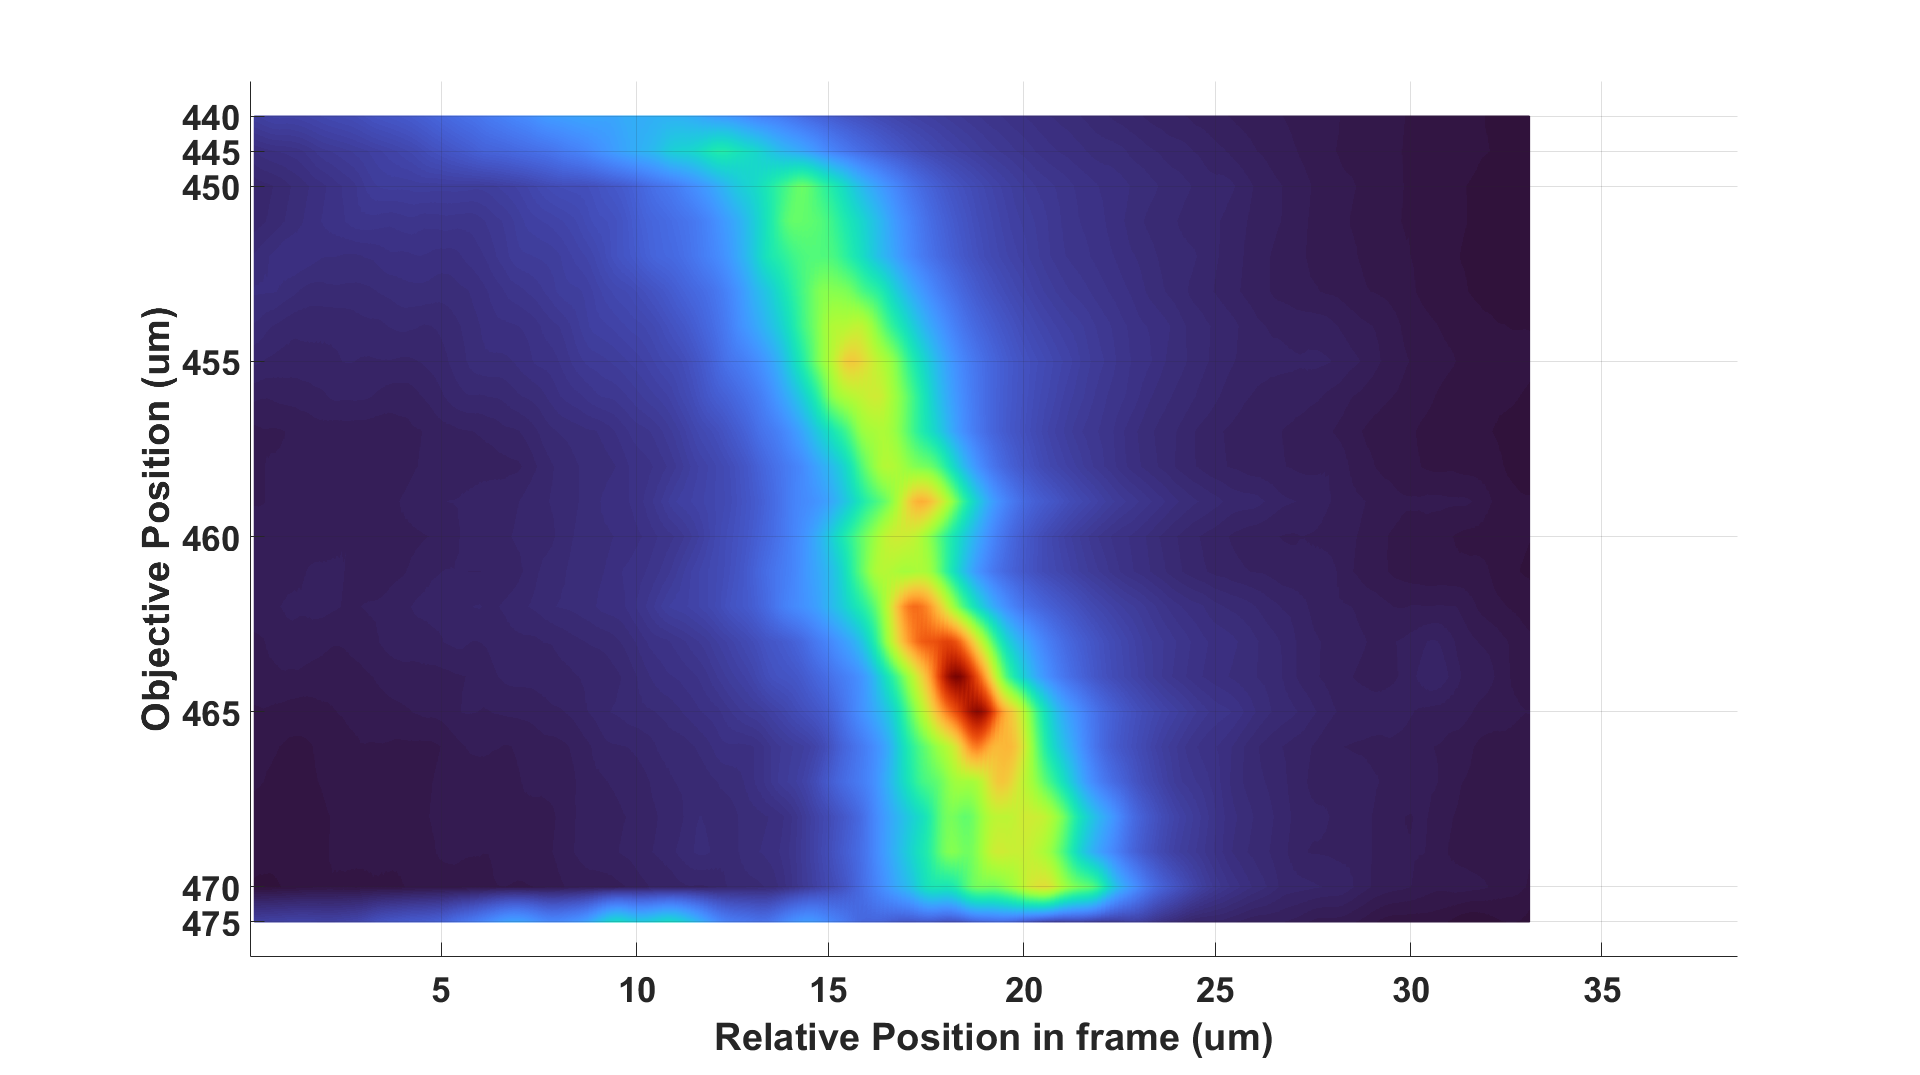
\includegraphics[width=\textwidth]{LS_Heatmap.png}
    \caption{This heatmap displays the intensity of the light sheet as a function of objective's position. Note how the sheet tapers in width and spikes in intensity around the focal plane of the light sheet circa objective position 464 microns. The drift of the light sheet as the objective is translated updwards (down on the graph) shows the lightsheet is emerging at around $75^\circ$, rather than orthogonal to, the sample plane.}
\end{figure}




% \end{multicols}

% Insert Beam Characterization graph once it has been properly scaled!
\newpage
 \printbibliography[heading=bibintoc]

\end{document} 
